\chapter{Results}
\label{chap:results}

This chapter evaluates the proposed embedding-guided $A^*$ search for binary causal question answering, focusing on both effectiveness and search efficiency. The evaluation addresses four research questions. RQ1 assesses the impact of fine-tuning on the embedding heuristic, while RQ2 analyzes the role of Matryoshka dimensionality. RQ3 compares the selected $A^*$ configuration with the BFS and RL baselines. Finally, RQ4 evaluates its generalization across different datasets and causal graph variants.

Section~\ref{sec:results-evaluation-setup} introduces the experimental setup and evaluation metrics. The subsequent analyses examine the effect of fine-tuning in Section~\ref{sec:results-finetuning} and Matryoshka dimensionality in Section~\ref{sec:results-matryoshka}, addressing RQ1 and RQ2, respectively. Section~\ref{sec:results-comparison} presents the final comparison with the baselines and evaluates performance across datasets and graph variants, addressing RQ3 and RQ4. Finally, Section~\ref{sec:results-ablation} concludes the analysis with an ablation study of the activation function and distance metric.

\section{Evaluation Setup}
\label{sec:results-evaluation-setup}

This section describes the evaluation procedure, datasets, causal graphs, models and baselines, and the methodology used throughout the experiments.

\subsection{Evaluation Procedure}
\label{sec:results-procedure}

The evaluation is organized in two stages. First, MS MARCO validation~\citep{nguyen:2016,bluebaum:2024} with CauseNet Precision~\citep{heindorf:2020} is used to analyze fine-tuning and Matryoshka dimensionality and select the final $A^*$ configuration. Second, the selected configuration is evaluated on the MS MARCO and SemEval~\citep{hendrickx:2010,sharp:2016,bluebaum:2024} test splits across CauseNet Precision, CauseNet Full~\citep{heindorf:2020}, and CEG Filtered~\citep{li:2020}, and compared with BFS and the RL approach of \citet{bluebaum:2024}.

\subsection{Datasets}
\label{sec:results-datasets}

The causal question answering datasets used in this thesis are derived subsets rather than the complete original datasets. The MS MARCO data are based on causal questions extracted from the original MS MARCO dataset~\citep{nguyen:2016} as part of Webis-CausalQA-22~\citep{bondarenko:2022}, while the SemEval data are based on the causal-relation subset of SemEval-2010 Task 8~\citep{hendrickx:2010} introduced by \citet{sharp:2016}. The binary causal splits for both datasets were provided by \citet{bluebaum:2024}. During evaluation, examples are skipped if the potential cause, the effect, or both are absent from the evaluated graph. Table~\ref{tab:dataset-statistics} reports the dataset sizes and class distributions in the original splits and after graph-node coverage filtering. Because graph-node coverage differs across graphs, each graph is evaluated on a different subset of questions with a different class distribution. Differences in effectiveness across graphs should therefore not be attributed solely to the graph itself.

\begin{table}[t]
\centering
\small
\setlength{\tabcolsep}{6pt}
\caption{Number of causal questions in MS MARCO and SemEval before and after graph-node coverage filtering. ``Total'' counts all causal samples in each local split. The graph columns count samples where both the potential cause and effect are covered by the corresponding graph.}
\label{tab:dataset-statistics}
\begin{tabular}{@{}p{2.75cm}rrrrrrrr@{}}
\toprule
\textbf{Split}
& \multicolumn{2}{c}{\textbf{Total}}
& \multicolumn{2}{c}{\textbf{CauseNet\textsubscript{Prec}}}
& \multicolumn{2}{c}{\textbf{CauseNet\textsubscript{Full}}}
& \multicolumn{2}{c}{\textbf{CEG\textsubscript{Filtered}}} \\
\cmidrule(lr){2-3}
\cmidrule(lr){4-5}
\cmidrule(lr){6-7}
\cmidrule(l){8-9}
& \textbf{Pos.} & \textbf{Neg.}
& \textbf{Pos.} & \textbf{Neg.}
& \textbf{Pos.} & \textbf{Neg.}
& \textbf{Pos.} & \textbf{Neg.} \\
\midrule
\multicolumn{9}{@{}l}{MS MARCO \citep{nguyen:2016,bluebaum:2024}} \\
Train      & $1{,}837$ & $0$  & $1{,}213$ & $0$  & $1{,}618$ & $0$  & $389$ & $0$ \\
Validation & $194$     & $47$ & $137$     & $22$ & $176$     & $35$ & $44$  & $8$ \\
Test       & $223$     & $40$ & $143$     & $20$ & $189$     & $31$ & $41$  & $7$ \\
\addlinespace[2pt]
\multicolumn{9}{@{}l}{SemEval \citep{hendrickx:2010,sharp:2016,bluebaum:2024}} \\
Train      & $694$ & $690$ & $541$ & $177$ & $680$ & $615$ & $496$ & $416$ \\
Validation & $84$  & $89$  & $66$  & $28$  & $81$  & $77$  & $57$  & $65$ \\
Test       & $87$  & $86$  & $66$  & $24$  & $84$  & $76$  & $57$  & $53$ \\
\bottomrule
\end{tabular}
\end{table}


\subsection{Causal Graphs}
\label{sec:results-graphs}

The evaluation uses three graph settings. CauseNet Precision is the high-precision subset of CauseNet~\citep{heindorf:2020} and is used for training, validation, model selection, and the main comparison to prior work. CauseNet Full is used to test scalability to a substantially larger graph. The third evaluated graph is a filtered version of the original CEG~\citep{li:2020}. Because CEG is very dense and contains many low-confidence edges, filtering is applied using the causal-strength formulation of \citet{luo:2016}, which combines necessity and sufficiency scores. For each CEG edge from cause \(c\) to effect \(e\), the causal strength is computed as\looseness=-1
\[
    \mathrm{CS}(c,e)
    =
    \mathrm{necessity}(c,e)^{\lambda}
    \cdot
    \mathrm{sufficiency}(c,e)^{1-\lambda},
\]
where \(\lambda\in[0,1]\) is a weighting parameter. This thesis uses \(\lambda = 0.9\), following \citeauthor{luo:2016}, and retains only edges with \(\mathrm{CS}(c,e) \geq 0.1\). All graph files undergo the same preprocessing, which removes empty or punctuation-only concepts and self-loops and normalizes labels by replacing underscores with spaces and stripping surrounding whitespace. Table~\ref{tab:graph-statistics} reports the resulting graph sizes.\footnote{The publicly available CEG release, in which cause--effect pairs with a reported frequency of \(5\) or lower are already excluded, contains approximately \(92.3\) million edges. In contrast, the official CEG release documentation~\citep{li:2020} reports approximately \(89.1\) million cause--effect pairs for this version. The available release information is insufficient to determine the source of this discrepancy conclusively. The official CauseNet statistics report \(199{,}806\) relations and \(80{,}223\) concepts for CauseNet Precision and \(11{,}609{,}890\) relations and \(12{,}186{,}195\) concepts for CauseNet Full~\citep{heindorf:2020}. The slightly smaller counts in Table~\ref{tab:graph-statistics} result from the preprocessing used in this thesis, which removes empty or punctuation-only concepts and self-loops and normalizes concept labels.}

\begin{table}[t]
  \centering
  \small
  \begin{tabular}{@{}p{9.65cm}rr@{}}
    \toprule
    \textbf{Graph} & \textbf{Nodes} & \textbf{Edges} \\
    \midrule
    CauseNet Precision & $80{,}211$ & $197{,}370$ \\
    CauseNet Full & $12{,}185{,}890$ & $11{,}606{,}919$ \\
    CEG Filtered & $77{,}264$ & $21{,}507{,}177$ \\
    CEG & $79{,}865$ & $92{,}270{,}736$ \\
    \bottomrule
  \end{tabular}
  \caption{Number of nodes and unique directed edges after graph preprocessing. CEG is reported for reference, while CEG Filtered is used in the evaluation.}
  \label{tab:graph-statistics}
\end{table}


\subsection{Models and Baselines}
\label{sec:results-models}

For embedding-guided \(A^*\), five embedding backbones are evaluated alongside the RL baseline of \citet{bluebaum:2024}. The \(A^*\) models and RL policy are trained using the MS MARCO training split and CauseNet Precision. Unlike the original RL setup, the policy is trained and evaluated without inverse edges because these may introduce transitions that do not represent causality in the queried direction. This ensures that all methods operate on the same forward directed-reachability task. Table~\ref{tab:model-overview} defines the model identifiers, parameter counts, embedding dimensions, and concise labels used throughout the results. Table~\ref{tab:training-hyperparameters} reports the selected hyperparameters and final training epoch for each fine-tuned embedding model. The epoch denotes the zero-indexed last validation improvement before early stopping with a patience of 10. The checkpoint from this epoch is retained as the final model.


\begin{table}[t]
\centering
\footnotesize
\setlength{\tabcolsep}{4pt}
\caption{Models used in the evaluation. The table reports the model labels used throughout this thesis, the corresponding model identifiers, parameter counts, and native embedding dimensions $d$.}
\label{tab:model-overview}
\begin{tabular}{@{}p{3.55cm}p{7.45cm}r r@{}}
\toprule
\textbf{Model label} & \textbf{Model identifier} & \textbf{Params.} & $\boldsymbol{d}$ \\
\midrule
RL \citep{bluebaum:2024}
& LSTM policy model
& 12M & -- \\

MPNet \citep{song:2020mpnet,allmpnet:modelcard}
& \texttt{sentence-transformers/all-mpnet-base-v2}
& 109M & 768 \\

BGE \citep{xiao:2024,bge:modelcard}
& \texttt{BAAI/bge-large-en-v1.5}
& 335M & 1024 \\

Granite \citep{awasthy:2025graniter2,granite:modelcard}
& \texttt{ibm-granite/granite-embedding-english-r2}
& 149M & 768 \\

mxbai \citep{mixedbread:2024mxbai,mxbai:modelcard}
& \texttt{mixedbread-ai/mxbai-embed-large-v1}
& 335M & 1024 \\

Qwen \citep{zhang:2025qwen3embedding,qwen3:modelcard}
& \texttt{Qwen/Qwen3-Embedding-0.6B}
& 0.6B & 1024 \\
\bottomrule
\end{tabular}
\end{table}

\begin{table}[t]
  \centering
  \small
  \begin{tabular}{@{}c@{\hspace{7.25em}}c@{}}
    \textbf{(a) Selected hyperparameters} & \textbf{(b) Selected epoch} \\[2pt]
    \begin{tabular}[t]{@{}lllr@{}}
      \toprule
      \textbf{Model} & \textbf{Activation} & \textbf{Metric} & \textbf{lr [$10^{-5}$]} \\
      \midrule
      MPNet & ReLU & Cosine & $2.673$ \\
      BGE & ReLU & Cosine & $2.924$ \\
      mxbai & ReLU & Cosine & $2.935$ \\
      Granite & ReLU & Euclidean & $2.709$ \\
      Qwen & ReLU & Cosine & $2.887$ \\
      \bottomrule
    \end{tabular}
    &
    \begin{tabular}[t]{@{}lr@{}}
      \toprule
      \textbf{Model} & \textbf{Epoch} \\
      \midrule
      MPNet & 0 \\
      BGE & 0 \\
      mxbai & 3 \\
      Granite & 10 \\
      Qwen & 10 \\
      \bottomrule
    \end{tabular}
  \end{tabular}
  \caption{Final training settings. Panel (a) reports the selected activation function, distance metric, and learning rate. Panel (b) reports the zero-indexed epoch of the last improvement in validation $A^*$ cost. Its checkpoint is retained for evaluation.}
  \label{tab:training-hyperparameters}
\end{table}


\subsection{Evaluation Methodology}
\label{sec:results-methodology}

This section describes the experimental evaluation, including search budgets, metrics, runtime measurement, model selection, and significance testing.

\subsubsection{Search Budgets}

The evaluation reports two BFS variants and budgeted \(A^*\). BFS (uncapped) runs without a visit limit and serves as the exhaustive reachability baseline. For BFS (capped) and \(A^*\), budgets are set to the 95th percentile ($p_{95}$) of visited nodes from successful searches on the MS MARCO training split with CauseNet Precision. BFS uses one global cap, whereas \(A^*\) uses separate budgets for each embedding model and Matryoshka dimension, as reported in Table~\ref{tab:p95-visited-nodes}. Uncapped \(A^*\) is additionally reported in the fine-tuning analysis to separate the effect of fine-tuning from the visit budget. The Matryoshka and final evaluations use the budgeted variants. Following the implementation of \citet{bluebaum:2024}, RL has no visit budget and instead uses beam search with a beam width of \(50\), a \textsc{stay} action, and a rollout length of two.

\begin{table}[H]
\centering
\small
\caption{$A^*$ visit budgets $\tau$ derived from the $p_{95}$ of visited nodes in successful searches on MS MARCO train with CauseNet Precision. Pretrained models are reported at their full embedding dimension, while fine-tuned models are reported across all evaluated Matryoshka dimensions.}
\label{tab:p95-visited-nodes}
\begin{tabular}{@{}p{2.39cm}rrrrrrrrrrr@{}}
\toprule
\textbf{Model} & \multicolumn{11}{c}{\textbf{Dimension}} \\
\cmidrule(l){2-12}
 & \textbf{2} & \textbf{4} & \textbf{8} & \textbf{16} & \textbf{32} & \textbf{64} & \textbf{128} & \textbf{256} & \textbf{512} & \textbf{768} & \textbf{1024} \\
\midrule
BGE & -- & -- & -- & -- & -- & -- & -- & -- & -- & -- & $379$ \\
BGE tuned & $682$ & $96$ & $27$ & $12$ & $10$ & $8$ & $8$ & $8$ & $9$ & $10$ & $10$ \\

Granite & -- & -- & -- & -- & -- & -- & -- & -- & -- & $825$ & -- \\
Granite tuned & $68$ & $16$ & $12$ & $13$ & $16$ & $23$ & $25$ & $23$ & $29$ & $32$ & -- \\

MPNet & -- & -- & -- & -- & -- & -- & -- & -- & -- & $503$ & -- \\
MPNet tuned & $1{,}120$ & $178$ & $41$ & $18$ & $13$ & $14$ & $15$ & $17$ & $21$ & $22$ & -- \\

mxbai & -- & -- & -- & -- & -- & -- & -- & -- & -- & -- & $376$ \\
mxbai tuned & $247$ & $62$ & $20$ & $12$ & $9$ & $8$ & $9$ & $9$ & $9$ & $9$ & $9$ \\

Qwen & -- & -- & -- & -- & -- & -- & -- & -- & -- & -- & $594$ \\
Qwen tuned & $253$ & $105$ & $10$ & $6$ & $5$ & $5$ & $5$ & $5$ & $5$ & $6$ & $5$ \\
\bottomrule
\end{tabular}
\end{table}


\subsubsection{Metrics}

Effectiveness is measured using precision, recall, and F\textsubscript{1}. Efficiency is measured using the average number of visited nodes and the average runtime per query in milliseconds. For BFS and \(A^*\), visited nodes count nodes processed during graph search, whereas for RL, following the original implementation, they count unique nodes in retained beam paths until the target is first encountered. Runtime additionally reflects neural inference, distance computation, and implementation overhead, whereas visited nodes provide a hardware-independent measure of traversal effort that is less sensitive to system load and hardware variation. The two metrics therefore capture complementary aspects of algorithmic search effort and practical execution cost.

\subsubsection{Runtime Measurement}

All evaluations were run on the Webis Slurm infrastructure using eight CPU cores, 128\,GB of memory, and one \texttt{H100} GPU.\footnote{Further details are available at \url{https://webis.de/facilities.html}.} Embedding computations use CUDA, while BFS runs on the CPU. Runtime is measured per query using Python's \texttt{time.perf\_counter()}, with CUDA synchronization before and after traversal. One untimed warm-up is performed per strategy. Graph loading, embedding precomputation, and cache loading are excluded, and reported runtimes are averages over a single evaluation run.

\subsubsection{Model Selection}

The final \(A^*\) configuration is selected from the capped fine-tuned validation results across all Matryoshka dimensions by balancing effectiveness and search efficiency. First, candidates dominated by another configuration with at least as high an F\textsubscript{1} score and no more visited nodes \(N\) are removed. Among the remaining candidates, a knee is selected, representing a point beyond which improving one objective requires a disproportionate deterioration in the other~\citep{branke:2004}. The selection adapts the normalized difference-curve construction of \citet{satopaa:2011}. F\textsubscript{1} and the logarithm of \(N\) are min--max normalized to $\widetilde{F_1}$ and $\widetilde{\log N}$, respectively. The score $(\widetilde{F_1}-\widetilde{\log N})/\sqrt{2}$ measures the signed perpendicular distance from the equal-trade-off diagonal, with larger values indicating a better combination of high F\textsubscript{1} and low search effort. The configuration with the largest score is selected. Runtime, the visit budget, and the embedding dimension are used only as tie-breakers, in that order.

\subsubsection{Statistical Significance Testing}

Statistical significance is tested only for the final test comparison. For each dataset--graph combination, the selected \(A^*\) configuration is compared with BFS (uncapped), BFS (capped), and RL using a paired stratified bootstrap test \citep{koehn:2004,dror:2018}. Positive and negative examples are resampled separately over \(10{,}000\) bootstrap samples. Bonferroni correction is applied to the three comparisons at a family-wise significance level of \(\alpha=0.05\). The reported p-values are Bonferroni-adjusted and compared with \(0.05\), whereas the 95\% confidence intervals remain unadjusted for each individual comparison.

\section{Effect of Fine-Tuning}
\label{sec:results-finetuning}

RQ1 asks whether fine-tuning improves the embedding heuristic used by $A^*$. Table~\ref{tab:validation-full-dim} compares each model before and after fine-tuning at its full embedding dimension on MS MARCO validation with CauseNet Precision, using the best hyperparameter configuration from Table~\ref{tab:training-hyperparameters}. The BFS variants and RL are included as references. RL appears only in the uncapped group because it has no visit budget, although its beam width and rollout length remain fixed. The capped runs use their respective $p_{95}$ budgets from MS MARCO train, whereas the uncapped runs remove the visit limit.

With the cap, pretrained embeddings reach F\textsubscript{1} scores between \(86.2\%\) and \(87.1\%\) while visiting 66.1 to 142.0 nodes on average. Fine-tuning reduces average visited nodes to between 3.5 and 11.0 and runtime for every model, but also lowers F\textsubscript{1} to between \(74.6\%\) and \(82.4\%\). Without the cap, all $A^*$ variants obtain the same F\textsubscript{1} of \(90.6\%\), as uncapped $A^*$ is complete. Fine-tuning nevertheless reduces visited nodes for all five models and runtime for BGE, Granite, MPNet, and Qwen. For mxbai, runtime increases slightly despite visiting fewer nodes on average, as a few unusually expensive searches raise the mean runtime. Thus, fine-tuning and visit budgets substantially improve search efficiency, while capped search trades some effectiveness for fewer visited nodes by terminating searches that exceed the budget.

Because the fine-tuned models use different $p_{95}$-derived budgets $\tau$, Figure~\ref{fig:budget-tradeoff} compares them at full dimensionality over a shared $\tau$ grid. MPNet provides the strongest trade-off across most of the range, followed by Granite and Qwen. mxbai requires more search effort for comparable F\textsubscript{1}, while BGE remains least effective. Larger budgets generally improve effectiveness by allowing $A^*$ to explore more nodes, but with diminishing returns.

\begin{table}[H]
\centering
\small
\setlength{\tabcolsep}{5pt}
\caption{Validation results on MS MARCO with CauseNet Precision at each model's full embedding dimension. Pretrained (PT) and fine-tuned (FT) $A^*$ are compared with BFS and RL under capped and uncapped search. Capped runs use their $p_{95}$ budget $\tau$. F\textsubscript{1} is reported in percent, N denotes average visited nodes, and T denotes runtime in milliseconds per query. The best value in each metric and search regime is bold, including ties.}
\label{tab:validation-full-dim}
\resizebox{\textwidth}{!}{%
\begin{tabular}{@{}llrrrrrrr@{}}
\toprule
& & & \multicolumn{3}{c}{\textbf{Capped}} & \multicolumn{3}{c}{\textbf{Uncapped}} \\
\cmidrule(lr){4-6}\cmidrule(lr){7-9}
\textbf{Model} & \textbf{Variant} & $\boldsymbol{\tau}$
& \textbf{F\textsubscript{1}} & \textbf{N} & \textbf{T}
& \textbf{F\textsubscript{1}} & \textbf{N} & \textbf{T} \\
\midrule
\multicolumn{2}{@{}l}{BFS}
& 1,316 & 86.6 & 184.8 & 0.7
& \textbf{90.6} & 1,659.8 & \textbf{2.2} \\
\multicolumn{2}{@{}l}{RL}
& -- & -- & -- & --
& 58.3 & \textbf{37.5} & 73.4 \\
\midrule
BGE & PT
& 379 & 86.6 & 68.6 & 9.1
& \textbf{90.6} & 1,342.4 & 41.5 \\
& FT
& 10 & 79.8 & 5.2 & 1.0
& \textbf{90.6} & 1,096.4 & 33.3 \\
Granite & PT
& 825 & 86.2 & 142.0 & 13.2
& \textbf{90.6} & 1,448.4 & 43.0 \\
& FT
& 32 & 82.3 & 11.0 & 1.9
& \textbf{90.6} & 1,252.8 & 29.8 \\
MPNet & PT
& 503 & 86.6 & 85.1 & 9.9
& \textbf{90.6} & 1,394.9 & 42.1 \\
& FT
& 22 & 82.4 & 7.5 & 1.7
& \textbf{90.6} & 1,101.4 & 34.2 \\
mxbai & PT
& 376 & 86.6 & 66.1 & 8.0
& \textbf{90.6} & 1,323.7 & 38.1 \\
& FT
& 9 & 74.6 & 5.2 & 0.9
& \textbf{90.6} & 1,259.3 & 40.1 \\
Qwen & PT
& 594 & \textbf{87.1} & 105.4 & 11.5
& \textbf{90.6} & 1,407.8 & 44.0 \\
& FT
& \textbf{5} & 78.4 & \textbf{3.5} & \textbf{0.6}
& \textbf{90.6} & 1,140.1 & 38.1 \\
\bottomrule
\end{tabular}%
}
\end{table}

\begin{figure}[t]
    \centering
    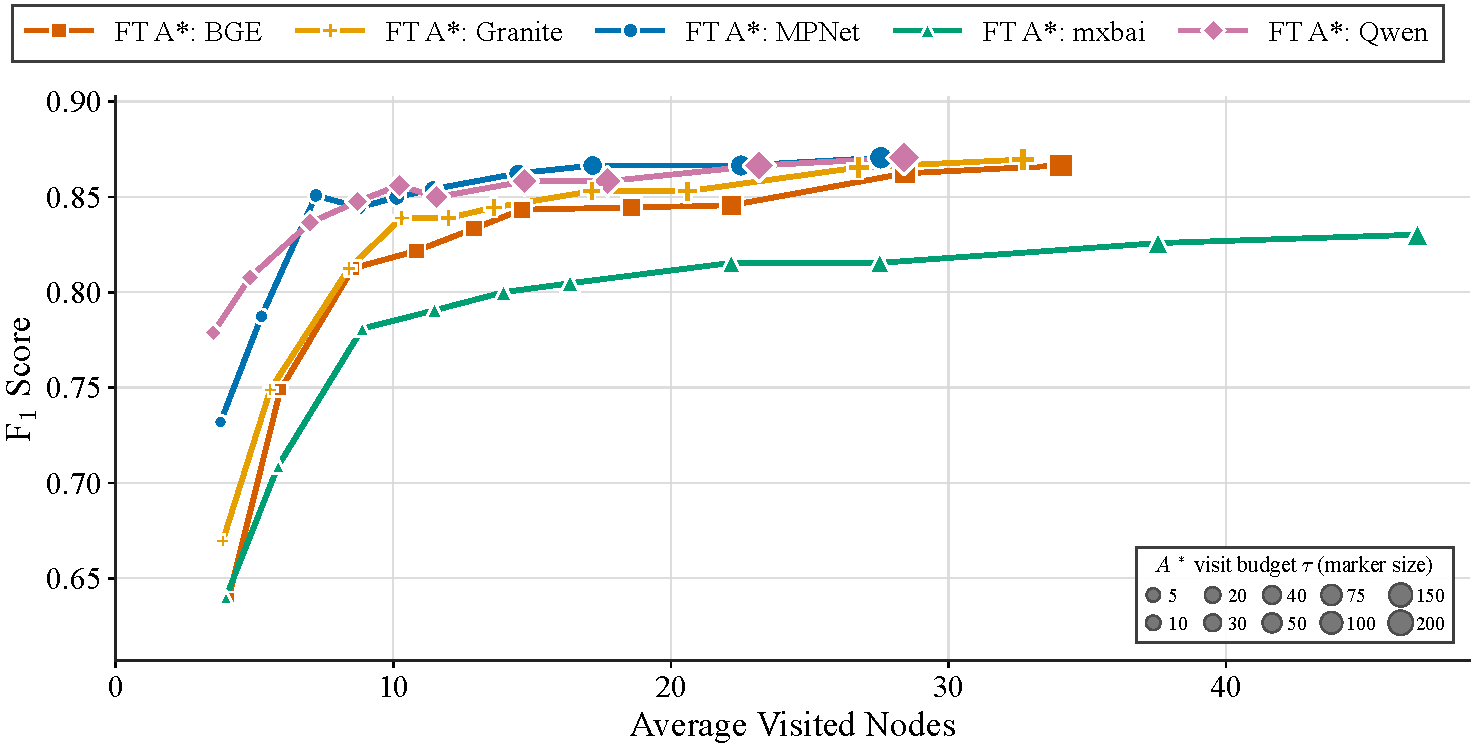
\includegraphics[width=\textwidth]{figures/budget_tradeoff_visited_nodes_linear.pdf}
    \caption{Efficiency--effectiveness trade-off for the five full-dimensional fine-tuned embedding models on MS MARCO validation with CauseNet Precision. F\textsubscript{1} score is shown against the measured average number of visited nodes, with marker size indicating the corresponding $A^*$ visit budget $\tau$.}
    \label{fig:budget-tradeoff}
\end{figure}

\section{Effect of Matryoshka Dimensionality}
\label{sec:results-matryoshka}

RQ2 examines the trade-off between effectiveness and efficiency across Matryoshka embedding dimensions. Figure~\ref{fig:metrics_summary} reports only capped fine-tuned models, using the same $p_{95}$-budget procedure across dimensions. Lower dimensions often reduce the visit budget, search effort, and runtime, although the effect is model-dependent and non-monotonic. For Granite, reducing the full 768-dimensional embedding to 32 dimensions lowers $\tau$ from 32 to 16, visited nodes from 11.0 to 7.1, and runtime from 1.9 to 1.2\,ms, while F\textsubscript{1} changes only slightly from \(82.3\%\) to \(81.9\%\). At 64 dimensions, F\textsubscript{1} instead improves to \(83.5\%\), with $\tau=23$, 9.1 visited nodes, and a runtime of 1.5\,ms. MPNet shows a similar intermediate optimum. At 64 dimensions, it retains the full model's \(82.4\%\) F\textsubscript{1} while reducing $\tau$ from 22 to 14, visited nodes from 7.5 to 6.1, and runtime from 1.7 to 1.3\,ms. Its two- and four-dimensional prefixes achieve higher F\textsubscript{1} scores of \(86.5\%\) and \(84.8\%\), but require 223.8 and 45.8 visited nodes, showing that lower dimensionality does not necessarily yield more efficient search. This instability at very low dimensions also appears for BGE and mxbai. Their two-dimensional variants reach \(83.6\%\) and \(79.2\%\) F\textsubscript{1}, respectively, but require 164.2 and 78.2 visited nodes. Qwen lies at the efficiency-oriented end of the trade-off, requiring only 3.8 visited nodes and 0.7\,ms at 768 dimensions, but reaching \(79.4\%\) F\textsubscript{1}. Different prefixes alter the embedding distances and therefore the order in which $A^*$ explores nodes. This helps explain why reducing dimensionality does not consistently reduce search effort. Overall, intermediate dimensions can provide better operating points than either the full embedding or very short prefixes while retaining sufficient information for effective search.

Among these operating points, MPNet-64 is the closest efficiency-oriented alternative to Granite-64, saving 2.9 node visits and 0.24\,ms while losing 1.1 percentage points of F\textsubscript{1}. On the global frontier, Granite-64 consequently obtains the higher Pareto-knee score, 0.285 compared with 0.257 for MPNet-64. Under the balanced effectiveness--efficiency objective, this effectiveness gain outweighs the modest additional search cost. MPNet-64, or Qwen-768 under a stricter latency constraint, could nevertheless be preferable when efficiency is prioritized more strongly. For the stated objective, the fine-tuned Granite-64 configuration with $\tau=23$ provides the best overall operating point and is therefore selected for the final test evaluation.

\begin{figure}[H]
    \centering
    \makebox[\textwidth][c]{%
        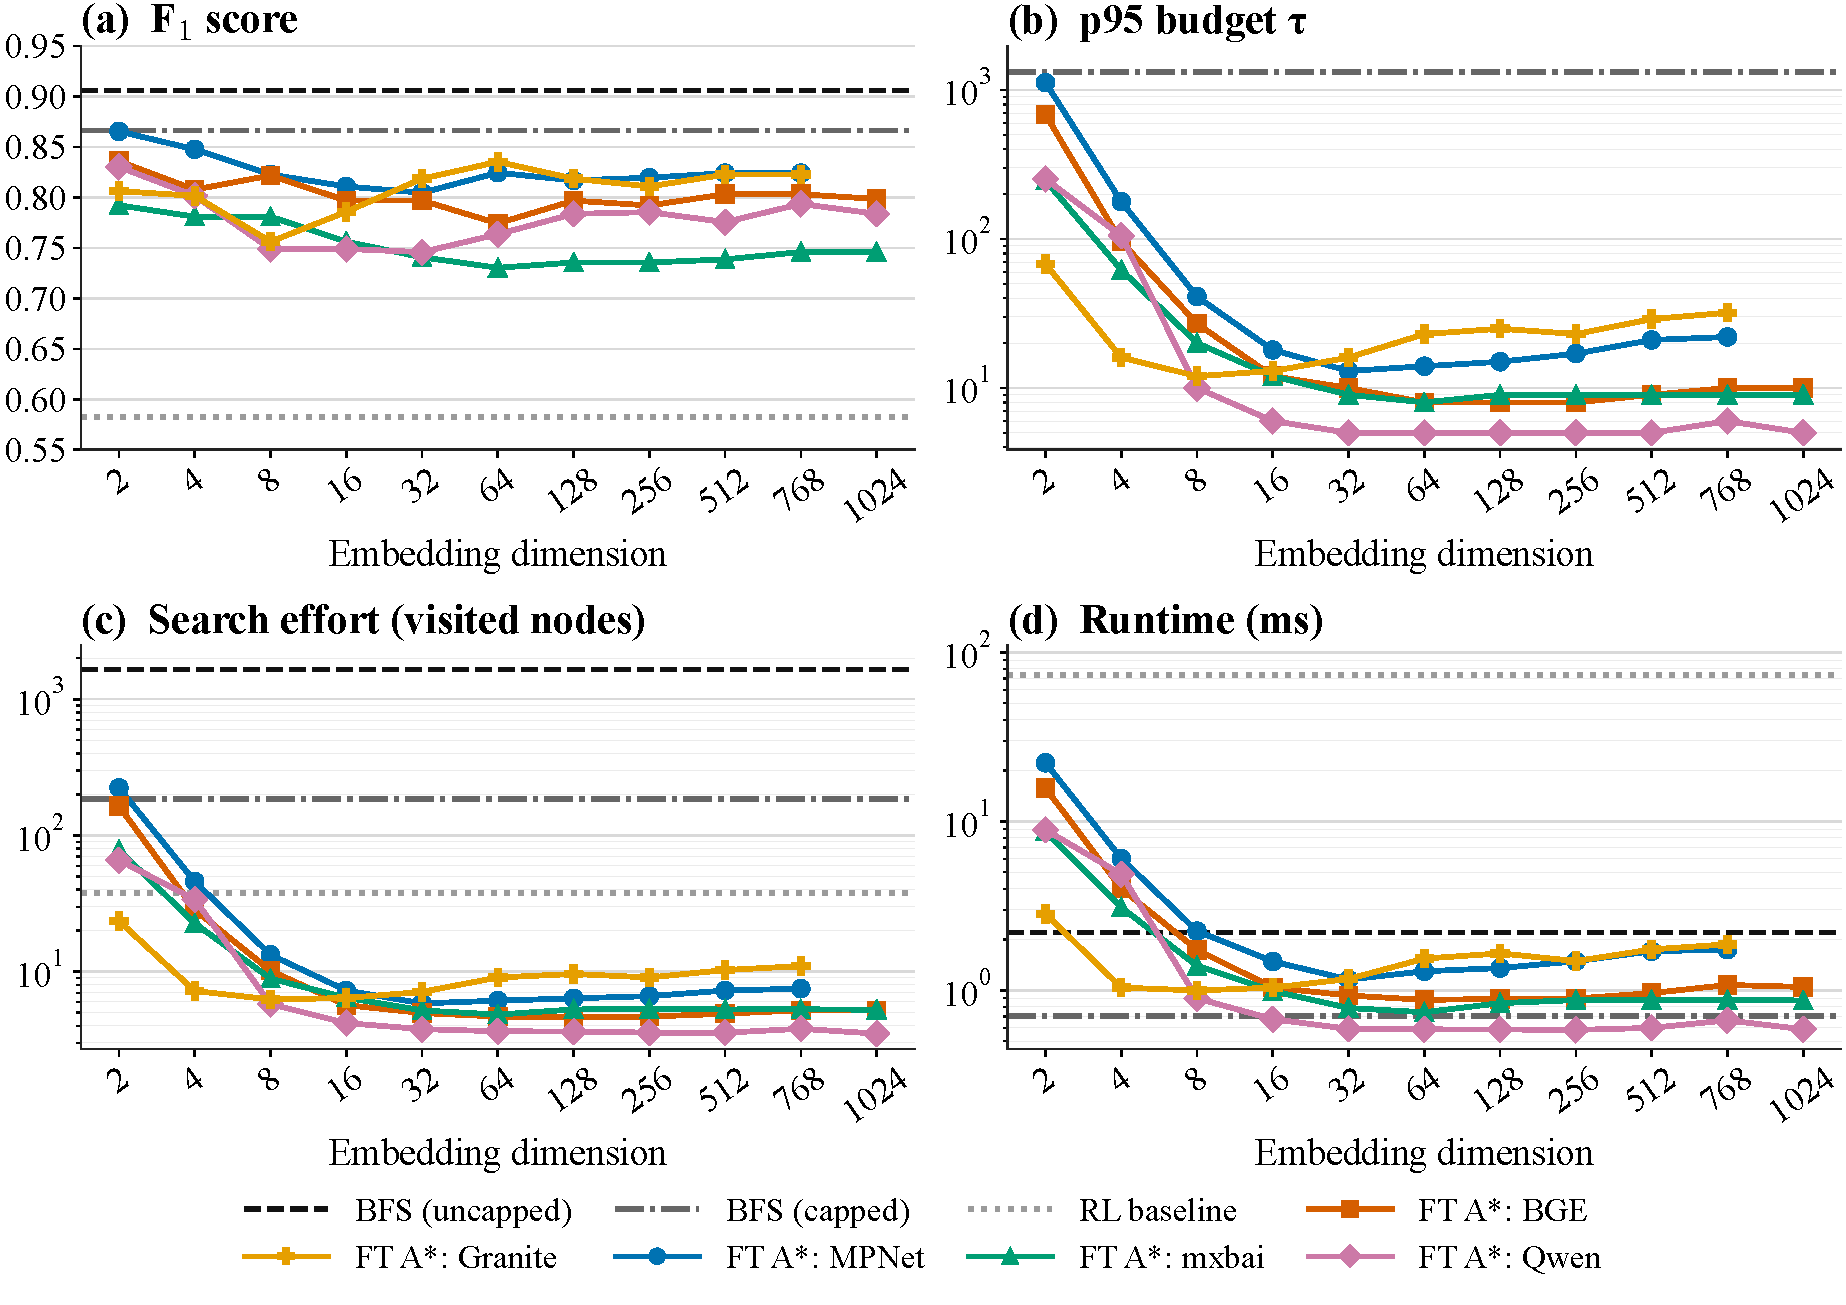
\includegraphics[width=1.05\textwidth]{figures/causenet_msmarco_valid_thesis_main.pdf}%
    }
        \caption{Validation performance of capped fine-tuned models on MS MARCO with CauseNet Precision across Matryoshka embedding dimensions. Shown are F\textsubscript{1}, the $p_{95}$ visit budget $\tau$, average visited nodes, and runtime. The budget, visited nodes, and runtime use logarithmic vertical axes.}
    \label{fig:metrics_summary}
\end{figure}

\section{Final Test Results}
\label{sec:results-comparison}

RQ3 compares the selected $A^*$ configuration with the BFS and RL baselines, while RQ4 examines its generalization across datasets and causal graph variants. Table~\ref{tab:final-results} reports the results on MS MARCO and SemEval for \mbox{CauseNet Precision}, CauseNet Full, and CEG Filtered. $A^*$ achieves a higher F\textsubscript{1} score, visits fewer nodes, and has a lower runtime than RL in all six settings. The comparison with BFS instead reveals an effectiveness--efficiency trade-off. On the smaller CauseNet Precision graph, BFS achieves the highest F\textsubscript{1} score on both datasets, whereas $A^*$ visits only 6.5 nodes on MS MARCO and 11.4 on SemEval. Capped BFS is faster in these settings, but visits 20.6 and 38.3 times as many nodes, respectively. This suggests that on smaller graphs, the overhead of embedding guidance can outweigh its savings in graph exploration.

On the larger CauseNet Full and denser CEG Filtered, the benefits of guided search become more pronounced. On CauseNet Full, $A^*$ visits only 7.5 nodes on MS MARCO and 14.2 on SemEval, compared with 30,099.3 and 160,715.3 for uncapped BFS. On MS MARCO, this substantial reduction in search effort comes with a lower F\textsubscript{1} score than either BFS variant. On SemEval, however, $A^*$ exceeds uncapped BFS by 9.5 percentage points and trails capped BFS by only 0.6 points. On CEG Filtered, $A^*$ attains an F\textsubscript{1} score of \(92.0\%\) on MS MARCO, matching capped BFS and slightly exceeding uncapped BFS while visiting only 2.3 nodes on average. Its F\textsubscript{1} score of \(68.5\%\) on SemEval lies between those of the two BFS variants, again with substantially fewer visited nodes and a lower runtime. These results demonstrate generalization beyond the CauseNet Precision--MS MARCO validation setting, with embedding guidance becoming more beneficial as graph exploration grows more expensive.

Tables~\ref{tab:f1-significance-causenet-precision}--\ref{tab:f1-significance-ceg} report paired stratified bootstrap tests for F\textsubscript{1} score differences between $A^*$ and each baseline. Positive $\Delta$ favors $A^*$ and negative $\Delta$ the baseline, with differences in percentage points. The 95\% confidence intervals are unadjusted, while $p_{\mathrm{Bonf.}}$ denotes the Bonferroni-adjusted $p$-value. The tests show that effectiveness depends on the graph and dataset. On MS MARCO, $A^*$ performs significantly worse than both BFS variants on \mbox{CauseNet Precision} and CauseNet Full, whereas neither comparison is significant on CEG Filtered. On SemEval, the pattern changes. $A^*$ significantly outperforms uncapped BFS on CauseNet Full, while its differences from both BFS variants on CauseNet Precision and capped BFS on CauseNet Full are not significant. The advantage over RL is more consistent, reaching significance on both datasets for both CauseNet variants, but not on CEG Filtered. Overall, the efficiency gains of $A^*$ do not imply a uniform loss in effectiveness. This is most apparent on CauseNet Full, where $A^*$ reduces graph exploration by several orders of magnitude while remaining competitive with BFS and outperforming RL.

\begin{table}[H]
\centering
\small
\setlength{\tabcolsep}{5pt}
\caption{Paired stratified bootstrap significance tests on CauseNet Precision.}
\label{tab:f1-significance-causenet-precision}
\begin{tabular}{@{}p{4.2cm}lrrrr@{}}
\toprule
\textbf{Dataset} & \textbf{Baseline} & $\boldsymbol{\Delta}$ & \textbf{95\% CI} & $\boldsymbol{p_{\mathrm{Bonf.}}}$ & \textbf{Sig.} \\
\midrule
MS MARCO & BFS (uncapped) & $-3.9$ & $[-6.7,-1.6]$ & $0.0123$ & yes \\
MS MARCO & BFS (capped)   & $-3.5$ & $[-6.2,-1.1]$ & $0.0306$ & yes \\
MS MARCO & RL             & $+16.4$ & $[+10.9,+22.5]$ & $0.0003$ & yes \\
SemEval  & BFS (uncapped) & $-5.2$ & $[-11.1,-0.2]$ & $0.1839$ & no \\
SemEval  & BFS (capped)   & $-4.9$ & $[-10.0,-0.8]$ & $0.1209$ & no \\
SemEval  & RL             & $+16.0$ & $[+7.0,+26.1]$ & $0.0048$ & yes \\
\bottomrule
\end{tabular}
\end{table}

\begin{table}[H]
\centering
\small
\setlength{\tabcolsep}{5pt}
\caption{Paired stratified bootstrap significance tests on CauseNet Full.}
\label{tab:f1-significance-causenet-full}
\begin{tabular}{@{}p{4cm}lrrrr@{}}
\toprule
\textbf{Dataset} & \textbf{Baseline} & $\boldsymbol{\Delta}$ & \textbf{95\% CI} & $\boldsymbol{p_{\mathrm{Bonf.}}}$ & \textbf{Sig.} \\
\midrule
MS MARCO & BFS (uncapped) & $-7.1$ & $[-10.6,-4.0]$ & $0.0006$ & yes \\
MS MARCO & BFS (capped)   & $-4.3$ & $[-7.2,-1.8]$ & $0.0084$ & yes \\
MS MARCO & RL             & $+13.0$ & $[+8.3,+17.9]$ & $0.0003$ & yes \\
SemEval  & BFS (uncapped) & $+9.5$ & $[+2.5,+15.6]$ & $0.0171$ & yes \\
SemEval  & BFS (capped)   & $-0.6$ & $[-6.9,+5.0]$ & $1.0000$ & no \\
SemEval  & RL             & $+24.8$ & $[+14.5,+35.5]$ & $0.0003$ & yes \\
\bottomrule
\end{tabular}
\end{table}

\begin{table}[H]
\centering
\small
\setlength{\tabcolsep}{5pt}
\caption{Paired stratified bootstrap significance tests on CEG Filtered.}
\label{tab:f1-significance-ceg}
\begin{tabular}{@{}p{4.2cm}lrrrr@{}}
\toprule
\textbf{Dataset} & \textbf{Baseline} & $\boldsymbol{\Delta}$ & \textbf{95\% CI} & $\boldsymbol{p_{\mathrm{Bonf.}}}$ & \textbf{Sig.} \\
\midrule
MS MARCO & BFS (uncapped) & $+1.0$ & $[+0.0,+3.2]$ & $1.0000$ & no \\
MS MARCO & BFS (capped)   & $+0.0$ & $[+0.0,+0.0]$ & $1.0000$ & no \\
MS MARCO & RL             & $+7.3$ & $[+0.6,+15.7]$ & $0.1671$ & no \\
SemEval  & BFS (uncapped) & $-0.2$ & $[-5.5,+4.5]$ & $1.0000$ & no \\
SemEval  & BFS (capped)   & $+0.2$ & $[-4.6,+4.6]$ & $1.0000$ & no \\
SemEval  & RL             & $+8.3$ & $[-2.2,+20.0]$ & $0.4260$ & no \\
\bottomrule
\end{tabular}
\end{table}

\begin{table}[t]
\centering
\small
\setlength{\tabcolsep}{2pt}
\sisetup{detect-weight=true}
\caption{Final test results for the selected fine-tuned Granite-64 $A^*$ configuration with $\tau=23$, compared with uncapped BFS (BFS-U), capped BFS (BFS-C), and the reinforcement learning baseline. CauseNet Prec. denotes CauseNet Precision. Precision (P), recall (R), and F\textsubscript{1} are reported in percent. T denotes runtime in milliseconds per query and N the average number of visited nodes. Asterisks mark F\textsubscript{1} scores that differ significantly from the selected $A^*$ configuration within each dataset--graph setting using a paired stratified bootstrap test with Bonferroni correction. Bold indicates the best value in each metric and dataset--graph setting, including ties.}
\label{tab:final-results}
\resizebox{\textwidth}{!}{%
\begin{tabular}{@{}llrrrrr@{\hspace{8pt}}rrrrr@{}}
\toprule
& & \multicolumn{5}{c}{\textbf{MS MARCO}} & \multicolumn{5}{c}{\textbf{SemEval}} \\
\cmidrule(lr){3-7}\cmidrule(lr){8-12}
\textbf{Graph} & \textbf{Approach}
& {\textbf{P}} & {\textbf{R}} & {\textbf{F\textsubscript{1}}} & {\textbf{T}} & {\textbf{N}}
& {\textbf{P}} & {\textbf{R}} & {\textbf{F\textsubscript{1}}} & {\textbf{T}} & {\textbf{N}} \\
\midrule
CauseNet Prec. & BFS-U
& 87.1 & {\bfseries 94.4} & {\bfseries 90.6$^{*}$} & 1.4 & 1157.3
& 89.2 & {\bfseries 87.9} & {\bfseries 88.5} & 6.6 & 6332.2 \\
CauseNet Prec. & BFS-C
& 87.5 & 93.0 & 90.2$^{*}$ & {\bfseries 0.5} & 134.9
& 91.8 & 84.8 & 88.2 & {\bfseries 1.2} & 436.7 \\
CauseNet Prec. & RL
& {\bfseries 89.2} & 58.0 & 70.3$^{*}$ & 67.7 & 32.0
& {\bfseries 97.1} & 51.5 & 67.3$^{*}$ & 114.4 & 38.3 \\
CauseNet Prec. & $A^*$
& 86.7 & 86.7 & 86.7 & 1.1 & {\bfseries 6.5}
& 92.6 & 75.8 & 83.3 & 1.8 & {\bfseries 11.4} \\
\midrule
CauseNet Full & BFS-U
& 85.6 & {\bfseries 94.7} & {\bfseries 89.9$^{*}$} & 59.5 & 30099.3
& 56.3 & {\bfseries 95.2} & 70.8$^{*}$ & 294.1 & 160715.3 \\
CauseNet Full & BFS-C
& 86.1 & 88.4 & 87.2$^{*}$ & 9.4 & 135.1
& 73.1 & 90.5 & {\bfseries 80.9} & 28.4 & 450.8 \\
CauseNet Full & RL
& {\bfseries 88.6} & 57.7 & 69.9$^{*}$ & 658.1 & 44.6
& {\bfseries 94.3} & 39.3 & 55.5$^{*}$ & 885.1 & 52.7 \\
CauseNet Full & $A^*$
& 86.7 & 79.4 & 82.9 & {\bfseries 7.2} & {\bfseries 7.5}
& 86.3 & 75.0 & 80.3 & {\bfseries 15.6} & {\bfseries 14.2} \\
\midrule
CEG Filtered & BFS-U
& 85.1 & {\bfseries 97.6} & 90.9 & 44.3 & 492.1
& 52.8 & {\bfseries 98.2} & {\bfseries 68.7} & 45.5 & 776.2 \\
CEG Filtered & BFS-C
& 87.0 & {\bfseries 97.6} & {\bfseries 92.0} & 5.8 & 30.2
& 52.9 & 96.5 & 68.3 & 9.1 & 42.4 \\
CEG Filtered & RL
& {\bfseries 89.2} & 80.5 & 84.6 & 5129.0 & 24.3
& {\bfseries 77.8} & 49.1 & 60.2 & 5131.9 & 54.7 \\
CEG Filtered & $A^*$
& 87.0 & {\bfseries 97.6} & {\bfseries 92.0} & {\bfseries 0.8} & {\bfseries 2.3}
& 56.2 & 87.7 & 68.5 & {\bfseries 4.4} & {\bfseries 7.2} \\
\bottomrule
\end{tabular}%
}
\end{table}


\section{Activation and Distance Ablation}
\label{sec:results-ablation}

This section analyzes the effects of the activation function and distance metric during fine-tuning. The same Granite model is trained with all four combinations of the ReLU or GELU activation function and Euclidean or cosine distance, while keeping all other settings fixed. The ablation is evaluated on CauseNet Precision, CauseNet Full, and CEG Filtered with both test datasets, using the selected 64-dimensional Matryoshka prefix and \(A^*\) budget \(\tau=23\).

Table~\ref{tab:activation-distance-ablation} reports the complete ablation results, while Figure~\ref{fig:ablation-tradeoff} summarizes the relationship between F\textsubscript{1} and search effort. ReLU--Euclidean provides the strongest overall trade-off across the evaluated settings. On both CauseNet variants, it achieves the highest F\textsubscript{1} and the lowest number of visited nodes. The results on CEG Filtered are more mixed. With \mbox{MS MARCO}, ReLU--Euclidean achieves the lowest search effort while tying for the highest F\textsubscript{1}. With SemEval, GELU--Cosine achieves the highest F\textsubscript{1}, whereas ReLU--Euclidean requires the fewest visited nodes. These results indicate that the preferred activation and distance combination can vary across graphs and datasets, although \mbox{ReLU--Euclidean} is the most consistent across settings.

Small runtime differences from Table~\ref{tab:final-results} result from separate evaluation runs. Among the ablation configurations, GELU is fastest in four of the six settings, including both CauseNet Full evaluations, but these gains generally coincide with lower F\textsubscript{1} and more visited nodes. For example, \mbox{GELU--Cosine} reduces runtime from \(14.9\) to \(7.4\)\,ms on CauseNet Full with SemEval compared with ReLU--Euclidean, but loses \(4.3\) F\textsubscript{1} points and visits \(1.2\) more nodes. Overall, ReLU--Euclidean provides the most consistent effectiveness--efficiency trade-off despite the runtime advantages of GELU in some settings.

\begin{figure}[H]
    \centering
    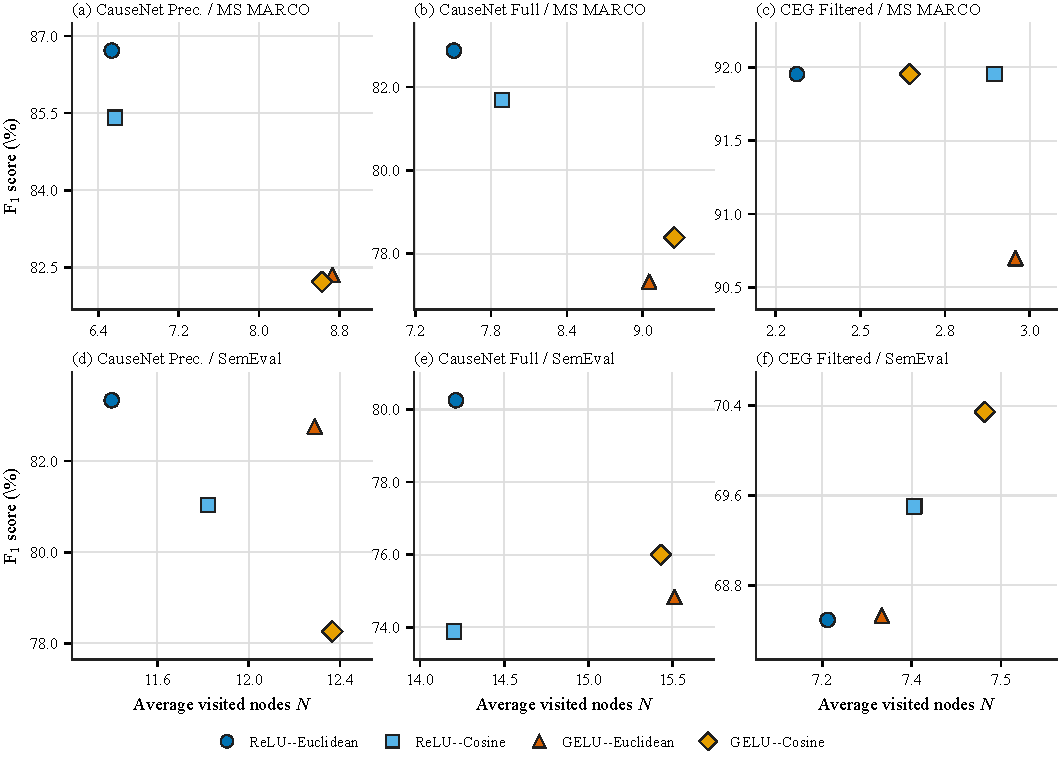
\includegraphics[width=\textwidth]{figures/ablation_tradeoff.pdf}
    \caption{Effectiveness--efficiency trade-off across activation and distance configurations. F\textsubscript{1} is plotted against average visited nodes across all six test settings.}
    \label{fig:ablation-tradeoff}
\end{figure}

\begin{table}[H]
\centering
\small
\setlength{\tabcolsep}{2pt}
\sisetup{detect-weight=true}
\caption{Activation and distance ablation for Granite-64 across all test settings with $\tau=23$. Bold indicates the best value per metric and setting, including ties.}
\label{tab:activation-distance-ablation}
\resizebox{\textwidth}{!}{%
\begin{tabular}{@{}ll
S[table-format=2.1]
S[table-format=2.1]
S[table-format=2.1]
S[table-format=2.1]
S[table-format=2.1]
@{\hspace{6pt}}
S[table-format=2.1]
S[table-format=2.1]
S[table-format=2.1]
S[table-format=2.1]
S[table-format=2.1]@{}}
\toprule
& & \multicolumn{5}{c}{\textbf{MS MARCO}}
& \multicolumn{5}{c}{\textbf{SemEval}} \\
\cmidrule(lr){3-7}\cmidrule(lr){8-12}
\textbf{Graph} & \textbf{Configuration}
& {\textbf{P}} & {\textbf{R}} & {\textbf{F\textsubscript{1}}} & {\textbf{T}} & {\textbf{N}}
& {\textbf{P}} & {\textbf{R}} & {\textbf{F\textsubscript{1}}} & {\textbf{T}} & {\textbf{N}} \\
\midrule
CauseNet Prec. & ReLU--Euclidean
& 86.7 & {\bfseries 86.7} & {\bfseries 86.7} & {\bfseries 1.0} & {\bfseries 6.5}
& 92.6 & {\bfseries 75.8} & {\bfseries 83.3} & 1.8 & {\bfseries 11.4} \\

CauseNet Prec. & ReLU--Cosine
& 87.0 & 83.9 & 85.4 & 1.1 & 6.6
& 94.0 & 71.2 & 81.0 & 1.9 & 11.8 \\

CauseNet Prec. & GELU--Euclidean
& 86.8 & 78.3 & 82.4 & 1.3 & 8.7
& {\bfseries 96.0} & 72.7 & 82.8 & {\bfseries 1.4} & 12.3 \\

CauseNet Prec. & GELU--Cosine
& {\bfseries 87.4} & 77.6 & 82.2 & 1.3 & 8.6
& 91.8 & 68.2 & 78.3 & 1.5 & 12.4 \\
\midrule

CauseNet Full & ReLU--Euclidean
& 86.7 & {\bfseries 79.4} & {\bfseries 82.9} & 6.9 & {\bfseries 7.5}
& 86.3 & {\bfseries 75.0} & {\bfseries 80.3} & 14.9 & {\bfseries 14.2} \\

CauseNet Full & ReLU--Cosine
& {\bfseries 87.3} & 76.7 & 81.7 & 6.5 & 7.9
& 79.5 & 69.0 & 73.9 & 12.3 & {\bfseries 14.2} \\

CauseNet Full & GELU--Euclidean
& 85.8 & 70.4 & 77.3 & 5.9 & 9.1
& {\bfseries 87.3} & 65.5 & 74.8 & 7.6 & 15.5 \\

CauseNet Full & GELU--Cosine
& 86.1 & 72.0 & 78.4 & {\bfseries 4.8} & 9.3
& 86.4 & 67.9 & 76.0 & {\bfseries 7.4} & 15.4 \\
\midrule

CEG Filtered & ReLU--Euclidean
& {\bfseries 87.0} & {\bfseries 97.6} & {\bfseries 92.0} & {\bfseries 0.8} & {\bfseries 2.3}
& 56.2 & 87.7 & 68.5 & 4.4 & {\bfseries 7.2} \\

CEG Filtered & ReLU--Cosine
& {\bfseries 87.0} & {\bfseries 97.6} & {\bfseries 92.0} & 1.4 & 2.9
& {\bfseries 58.3} & 86.0 & 69.5 & 4.4 & 7.4 \\

CEG Filtered & GELU--Euclidean
& 86.7 & 95.1 & 90.7 & 1.5 & 3.0
& 57.0 & 86.0 & 68.5 & {\bfseries 4.0} & 7.3 \\

CEG Filtered & GELU--Cosine
& {\bfseries 87.0} & {\bfseries 97.6} & {\bfseries 92.0} & 1.4 & 2.6
& 58.0 & {\bfseries 89.5} & {\bfseries 70.3} & 5.1 & 7.5 \\
\bottomrule
\end{tabular}%
}
\end{table}
